\documentclass[11pt,a4paper]{article}
\usepackage[utf8]{inputenc}
\usepackage[T1]{fontenc}
\usepackage{amsthm} %numéroter les questions
\usepackage[frenchb]{babel}
\usepackage{datetime}
\usepackage{xspace} % typographie IN
\usepackage{hyperref}% hyperliens
\usepackage[all]{hypcap} %lien pointe en haut des figures
\usepackage[french]{varioref} %voir x p y
\usepackage{fancyhdr}% en têtes
%\input cyracc.def
\usepackage[]{graphicx} %include pictures
\usepackage{pgfplots}
\usepackage[ ]{circuitikz}
\usepackage{ifthen}

\usepackage[top=1.3 in, bottom=1.3 in, left=1.3 in, right=1.3 in]{geometry} % Yeah, that's bad to play with margins
\usepackage[]{pdfpages}

\usepackage[]{attachfile}

\usepackage{float}

\newdateformat{mydate}{v1.0.0}%hack pour remplacer \THEYEAR


\newboolean{corrige}
\ifx\correction\undefined
\setboolean{corrige}{false}% pas de corrigé
\else
\setboolean{corrige}{true}%corrigé
\fi

\setboolean{corrige}{false}% pas de corrigé

\newboolean{annexes}
\setboolean{annexes}{true}%annexes
%\setboolean{annexes}{false}% pas de annexes

\definecolor{darkblue}{rgb}{0,0,0.5}

\newboolean{mos}
%\setboolean{mos}{true}%annexes
\setboolean{mos}{false}% pas de annexes

\usepackage{aeguill} %guillemets

%% fancy header & foot
\pagestyle{fancy}
%Numero du TP :
\def \labonumber {Laboratory work \no 2 }
\lhead{[ELEC-H-310] Digital Choucroute\\ \labonumber}
\rhead{\mydate\today\\ page \thepage}
\chead{\ifthenelse{\boolean{corrige}}{Corrigé}{}}
\cfoot{}
%%

\pdfinfo{
/Author (Quentin Delhaye, Ken Hasselmann, ULB -- BEAMS)
/Title (\labonumber ELEC-H-310)
/ModDate (D:\pdfdate)
}

\hypersetup{
pdftitle={\labonumber [ELEC-H-310] Digital Choucroute},
pdfauthor={Quentin Delhaye, Ken Hasselmann, ULB -- BEAMS},
pdfsubject={}
}

\theoremstyle{definition}% questions pas en italique
\newtheorem{Q}{Question}[] % numéroter les questions [section] ou non []

\newcommand{\reponse}[1]{% pour intégrer une réponse : \reponse{texte} : sera inclus si \boolean{corrige}
	\ifthenelse {\boolean{corrige}} {\paragraph{Answer :} \color{darkblue}   #1\color{black}} {}
 }

\newcommand{\addcontentslinenono}[4]{\addtocontents{#1}{\protect\contentsline{#2}{#3}{#4}{}}}

\date{\vspace{-1.7cm}\mydate\today}
\title{\vspace{-2cm} \labonumber\\ Digital Electronics [ELEC-H-310]\\Realization of a synthetizer\ifthenelse{\boolean{corrige}}{~\\Solution}{}}

%\author{\vspace{-1cm}}%\textsc{Yannick Allard}}

\setlength{\parskip}{0.2cm plus2mm minus1mm} %espacement entre §
\setlength{\parindent}{0pt}

\begin{document}
\pagestyle{empty}
\maketitle
% \vspace*{-1cm}
\section*{Purpose}
The main purpose of this manipulation is to create a complex digital system~: a sound synthetizer.
To implement it, you must understand the functioning of the analog-to-digital converter (ADC) as well as the digital-to-analog converter (DAC).

\section*{Prerequisite}
Before the lab, we advice you to read section 1 to 5 of the annex «~Programmation d’une carte à microcontrôleur~»

\section*{Predeterminations}
You are asked to answer exercices of section~\ref{sec:predet}.

\section*{Objectives}
At the end of this lab, you must be able to~:
\begin{itemize}
	\item Write a program for a microcontroller.
	\item Explain the functioning of an analog-to-digital converter.
	\item Explain the usefulness of the interrupt.
	\item Link the specifications to the peripherals of a microcontoller.
\end{itemize}

\newpage{}

\section{Introduction to the analog-to-digital conversion}

\subsection{Introduction}
Microprocessors are present in practically every industrial processes (temperature control, speed display, alarm systems) as well as in our common life (alarm-radio, audio systems, etc.).
All those processes have in common the interaction with analog variables (see figure~\ref{fig:arch-processus}).
Processors work with digital variables thus, it is necessary to convert those physical analog quantities into digital values and inversely.

The transformation of physical signal to digital is done in two steps~:
\begin{itemize}
	\item Conversion of the physical signal to measure (temperature, speed, ...) into voltage. It is the role of the sensor (thermocoupe, accelerometer, etc.).
	\item Conversion of this voltage into binary value. It is the role of the analog-to-digital converter (ADC).
\end{itemize}

The reversed path allows to convert a digital number to a physical quantity ~:
\begin{itemize}
	\item The digital-to-analog converter (DAC) transforms a binary number into voltage.
	\item The actuator converts the voltage into another physical quantity that will activate some system (\textit{e.g.} microwaves, electrical drives, gates, motors, etc.).
\end{itemize}

\begin{figure}[H]
	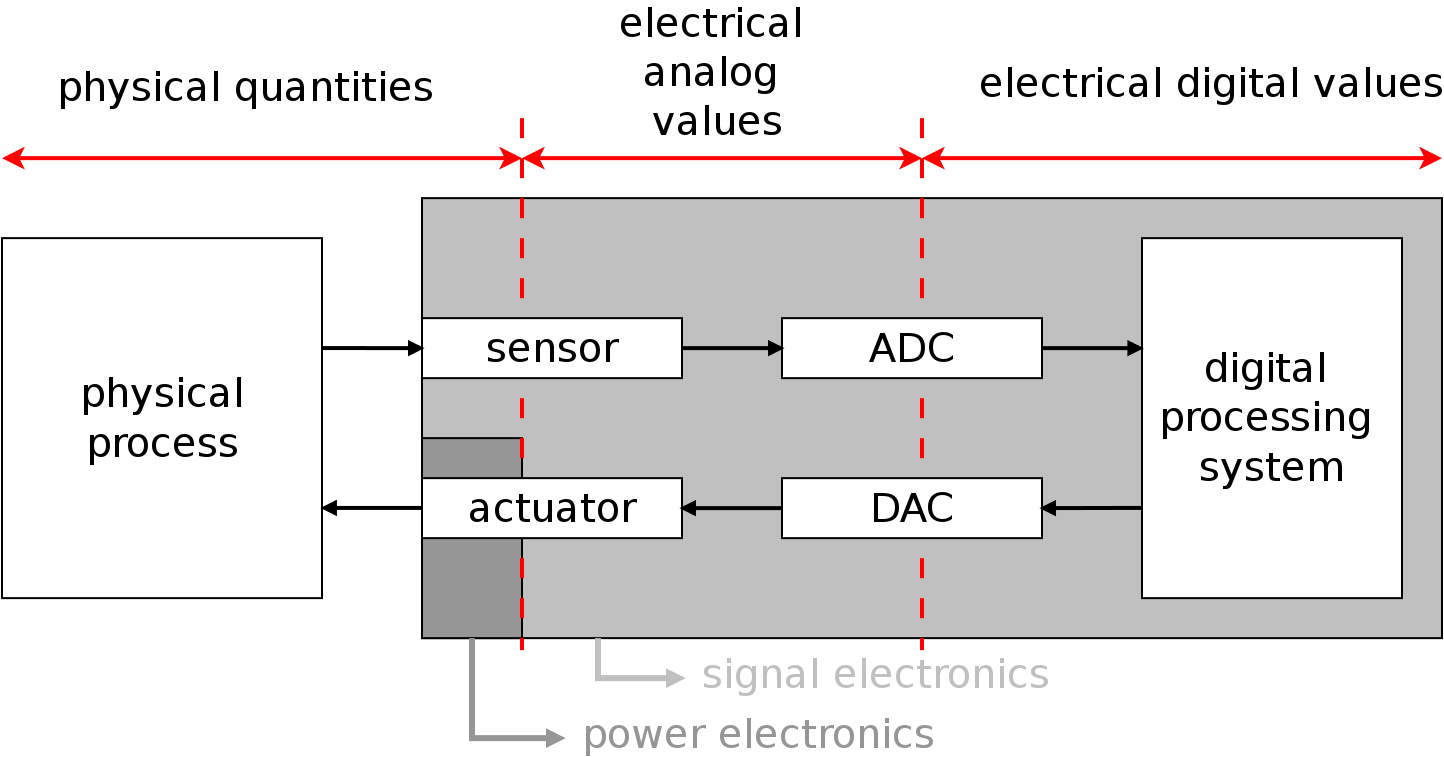
\includegraphics[width=\textwidth]{ENarch-processus}
	\caption{Architecture of a process}
	\label{fig:arch-processus}
\end{figure}

\subsection{Analog-to-digital conversion}
The analog-to-digital converter turns an analog voltage (changing continuously) into a digital number coded on a fixed value of bits (10 or 12 for the dsPIC).
To do so, the converter does a double quantization (see figure~\ref{fig:double-quant})~:
\begin{itemize}
	\item Time quantization, also called sampling.
	\item Level quantization.
\end{itemize}
Note that it is impossible to perfectly represent an analog signal into a finite number of bits.

\begin{figure}[H]
	\centering
	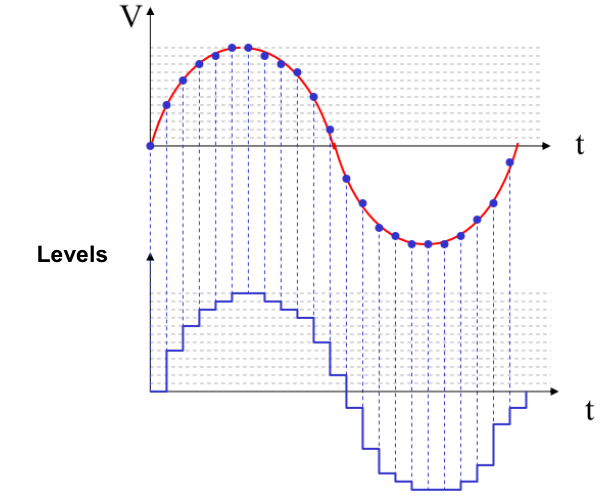
\includegraphics[width=.7\textwidth]{ENdouble-quant}
	\caption{Double quantization}
	\label{fig:double-quant}
\end{figure}

Performances of a DAC mostly depends on two parameters~:
\begin{itemize}
	\item The sampling frequency.
	\item The resolution, in other words the number N of bits coding the converted value.
    The resolution can be electrically defined as the smallest detectable change of voltage.
    If the converter has an operating range from 0~V to 5~V and convert the quantity on 10 bits, the resolution is $\frac{5 V}{2^{10}} = 4,9 mV$(\textit{i.e.} input range.
    Finally, each binary number coded on N bits will correspond to an input voltage range.

\end{itemize}

\begin{figure}
	\centering
	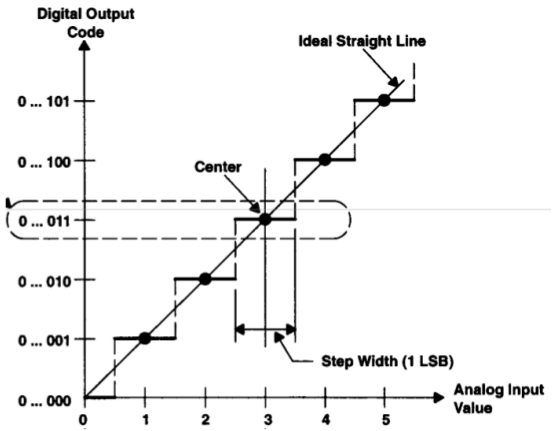
\includegraphics[width=.7\textwidth]{an-dig}
	\caption{Digital coding of an analog value}
	\label{fig:an-dig}
\end{figure}

\subsection{Digital-to-analog conversion}
Its principle is the opposite of the ADC~: the transformation of a number coded on N bits to a voltage in its output range.
The voltage obtained is continuous in time (the output of the converter is constant until a new conversion is done), but is always quantitized because only $2^N$ different voltage values are achievable (each binary code correspond to one voltage).



\section{Predeterminations}\label{sec:predet}
\begin{enumerate}
	\item Compute the resolution of ADC present on the Explorer16 board knowing that the input voltage range is 0-3,3V and that the ADC has 12 bits.
	\item Determine the memory space needed to store an audio file of 3s, sampled at 11kHz, knowing one sample is stored on one byte.
\end{enumerate}



\section{Manipulation}

\subsection{Realization of a voltmeter}
First of all, you will familiarize yourselves with the use of the ADC with a simple application~: a voltmeter measuring the voltage on a potentiometer connected to input \texttt{AN0}.
A feedback will be done using the LEDs as a bar graph (the higher the voltage, the more LEDs are switched on)
The bar graph must be updated at rate of 1~kHz.
\begin{itemize}
	\item Draw the block diagram of the whole system.
	Which peripheral will be used~?
    Highlight the interfaces between the inside and outside of the $\mu$C by seprating them clearly.
	\item Program ADC1 of the dsPIC. Somes lines of are already there for basic configuration of the ADC.
    Create a time base at predefined frequency. To link both the ADC and time base, you have the choice between several implementations~:
	\begin{itemize}
		\item Check the flag of the timer to launch the conversion, then look for the end-of-conversion flag (\texttt{IFS0bits.AD1IF}).
		\item Configure the ADC to launch automatically the conversion when the timer overflows.
        This is done by modifying the field \texttt{AD1CON1bits.SSRC} (cf. figure 32 in section 11 of the programming guide).
		Note~: in all cases, your function must not be blocking.
	\end{itemize}
	\item Realize the processing of the signal coming from the ADC \footnote{verify connection of potentiometer, see figure~\ref{fig:extension-board-jumper}}.
	\item Among all possible implementations, which ones guarantees the sampling period~?
\end{itemize}

\begin{figure}[h]
\centering
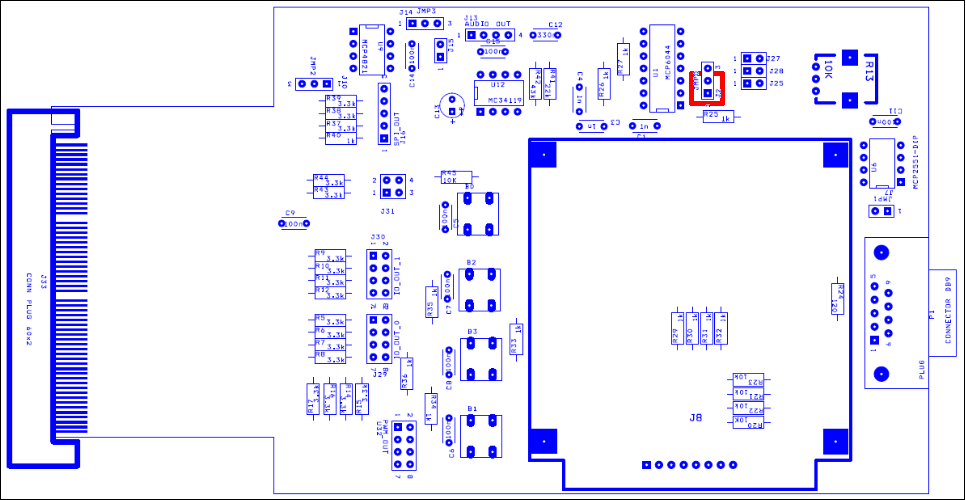
\includegraphics[width=0.9\textwidth]{extension-board-jumper}
\caption{Connect pin 1 and 2 of header \texttt{J2} with a jumper in order to connect the potentiometer to the input of the ADC.}
\label{fig:extension-board-jumper}
\end{figure}

\subsection{Synthetizer}
A synthetizer is a device capable of generating an arbitrary sound wave and convert it to sound through a speaker.
In our case, we will simply generate a sine wave at adjustable frequency~: the processor will send samples corresponding to the wanted waveform to a DAC and once rebuild, the signal will be send to the amplifier of the extension board.
\begin{itemize}
	\item Check that the line of code calling  \texttt{clav2LCD} is commented out.
	\item During the configuration of your peripherals (before the while loop), fill the wave vector defined as global variable so that it contains on full period of a sine wave defined between -2000 and 2000.
    To do so, you must~:
	\begin{itemize}
		\item include the file math.h in the header~;
		\item call function sin(), that takes as argument a floating number representing the angle (in rad) and that also returns a floating number.
	\end{itemize}
	\item Program a timer so that a sample of the sine wave is processed every 50~$\mu$s
	\item Play the sound through the speaker. The DAC is external and is accessible through the function \texttt{ecrit\_dac\_signal()}, defined in CNAserie.h and takes as argument an integer between 0 and 4095 (you must thus center your wave around 2048).
    With the help of the oscilloscope, check the waveform.
	\item Uncomment the line calling clav2LCD.
    Why is your program not working anymore~?
	\item Modify your program so that the processing is done in the interrupt routine of the timer.
    How does this solves the problem~?
	\item Add a volume control by coupling the measure from the potentiometer (representing the volume) with your synthetizer.
\end{itemize}



\end{document}
